\documentclass[a4,11pt]{aleph-notas}

%%--> Paquetes adicionales
\usepackage{enumitem}
\usepackage{textcomp}
\usepackage{multicol}

%%--> Preámbulo del material
%% --> Paquetes comunes
\usepackage{listings}
\usepackage{enumitem}
\usepackage{lipsum}

%% --> Definición de colores
\definecolor{codegreen}{HTML}{A5BE00}
\definecolor{codegray}{rgb}{0.5,0.5,0.5}
\definecolor{codepurple}{rgb}{0.58,0,0.82}
\definecolor{backcolour}{rgb}{0.95,0.95,0.92}

%% --> Estilo para código
\lstdefinestyle{mystyle}{
    language={[LaTeX]TeX}, % lenguaje
    basicstyle=\bfseries\ttfamily,
    keywordstyle=\color{colordef},
    commentstyle=\color{codegreen},
    backgroundcolor=\color{gray!15},
    showstringspaces=false,
    flexiblecolumns=true,
    stringstyle=\ttfamily\color{blue},
    extendedchars=true,
    emph={rm,bf,it,sf}, %...
    literate=%
    *{$}{{{\color{red}\$}}}1 % produce $ en rojo
    {$$}{{{\color{red}\$\$}}}1
    {ó}{{\'o}}1%
    {í}{{\'i}}1%
    {á}{{\'a}}1%
    {ú}{{\'u}}1%
}

%% --> Selección de estilo para el código
\lstset{
    style=mystyle,escapeinside={(*@}{@*)}
}

% Blancos tipográficos
\newcommand{\mq}{\hspace{0.5em}}  %medio cuadratín
\newcommand{\tq}{\hspace{0.33em}} % un terio de cuadratín
\newcommand{\qq}{\hspace{0.25em}} % un cuarto de cuadratín
\newcommand{\fs}{\hspace{0.125em}} % un octavo de cuadratín
\newcommand{\ep}{\hspace{0.05em}} % espacio de pelo

%% --> Nota para el material
\newcommand{\informacion}{\noindent\footnotesize{\color{colordef}
El presente material fue desarrollado por:

\noindent
\textbf{Daniel Lara}

\emph{Facultad de Ciencias, Escuela Politécnica Nacional}

\noindent
\textbf{Andrés Merino}

\emph{Facultad de Ciencias Exactas y Naturales, Pontificia Universidad Católica del Ecuador}


\medskip\noindent
La versión actual del material es 1.2-(Mayo 2021). En caso de encontrar inconsistencias o errores en el presente material se pueden comunicar a \href{mailto:daniel.lara@alephsub0.org}{daniel.lara@alephsub0.org}. Para más información puedes visitar nuestro sitio web: \href{https://alephsub0.org}{alephsub0.org}

\medskip\noindent

\includegraphics[height=12pt]{Imagenes/cc.xlarge.png} 
\includegraphics[height=12pt]{Imagenes/by.xlarge.png} 
\includegraphics[height=12pt]{Imagenes/nc.xlarge.png} \begin{minipage}[c]{0.85\textwidth}Esta obra se encuentra bajo licencia Atribución-NoComercial-CompartirIgual 4.0 Internacional (CC BY-NC-SA 4.0) Para más información puede visitar: \url{https://creativecommons.org/licenses/by-nc-sa/4.0/}\end{minipage}

\medskip\noindent
Si deseas colaborar con el desarrollo de este material, el código fuente está disponible en:   
\url{https://github.com/alephsub0/LaTeX_Guias.git}. Cualquier aporte (\emph{Pull request}) será de gran ayuda para mejorar este material. 

%% -- > Aquí se incluyen los nombres de los colaborades de estas guias:
\medskip\noindent
Agradecimientos: Katheryn Yánes
}}

%%--> Formato para títulos
\titleformat{name=\section,numberless}[display]
  {\vspace*{-2mm}\bfseries\scshape\centering}
    {}{1ex}
    {\color{colortext}\large\titlerule\vspace{.05ex}
     }
    [\color{colortext}\vspace{.2ex}\titlerule]

\titleformat{\subsubsection}
    {\color{colortext}\normalsize\bfseries}
    {\thesubsubsection}{1em}{}
    
%% --> Datos de las guias
\universidad{Curso de \LaTeX}
\autor{Proyecto Alephsub0}
\materia{Introducción a \LaTeX}

%% --> Logos de las guias
\logouno[4.5cm]{Imagenes/Logos/LogoAlephsub0-02.png}
\longtitulo{0.6\linewidth}
\fecha{Abril de 2021}

% -- Datos del libro
\nota{Guía 1}
\tema{Primeros pasos}
%%--> Opciones adicionales



%%%%%%%%%%%%%%%%%%%%%%%%%%%%%%%%%%%%%%%%
%%%%%%%%%% Comienzo del documento
%%%%%%%%%%%%%%%%%%%%%%%%%%%%%%%%%%%%%%%%

\begin{document}

\encabezado

\informacion

\tableofcontents

\section{Sitios web de utilidad}

Antes de comenzar el trabajo en \LaTeX{} es importante tomar en cuenta los siguientes enlaces para los recursos que nos serán de utilidad a lo largo del curso:

\begin{itemize}[leftmargin=*]
    \item
        Página de Overleaf: \url{https://www.overleaf.com/}
    \item
        Página oficial de \TeX Maker: \url{https://www.xm1math.net/texmaker/}
   \item
        Página oficial de MiK\TeX: \url{http://miktex.org/}
   \item
        Red de completa de archivos \TeX: \url{http://www.ctan.org/}
   \item 
        Catálogo en linea de paquetes de \LaTeX: \url{http://www.ctan.org/pkg/_A}
   \item
        Grupo de usuarios \TeX: \url{http://www.tug.org/}
    \item
        Comunidad de usuarios \LaTeX de Stack Exchange: \url{https://tex.stackexchange.com/}
\end{itemize}

\section{Atajos de teclado}

Una de las principales ventajas de \LaTeX{} es el uso casi exclusivo del teclado para el desarrollo de nuestro trabajo; así, es importante conocer algunas de las teclas de acceso rápido que se encuentran a nuestra disposición:

  \begin{itemize}
    \item \verb"Ctrl + enter" para compilar.
    \item \verb"Ctrl + /" para comentar el código.
    \item \verb@Ctrl + Home@ mueve al inicio del documento.
    \item \verb@Ctrl + End@ mueve al final del documento.
    \item \verb@Ctrl + L@ mueve a la linea especificada.
    \item \verb@Ctrl + D@ elimina la linea actual.
    \item \verb@Ctrl + B@ texto en negrita.
    \item \verb@Ctrl + I@ texto en itálica.
    \item \verb"Ctrl + F" para buscar y reemplazar.
    \item \verb"Ctrl + Shift + C" para agregar un comentario.
  \end{itemize}

\begin{advertencia}
Los atajos mostrados corresponden a \emph{Overleaf}. Una  lista completa se puede encontrar en: \href{https://es.overleaf.com/learn/how-to/Hotkeys}{https://es.overleaf.com/learn/how-to/Hotkeys}
\end{advertencia}

Para un trabajo eficiente se recomienda configurar adecuadamente el teclado, un video sobre este tema se puede encontrar a continuación: \href{https://youtu.be/btBeDseNiNc}{https://youtu.be/btBeDseNiNc}

\section{Primeros pasos}

\LaTeX \hspace{3pt} es una poderosa herramienta que compone textos en función de lineas de código. Al comportarse de manera análoga a un lenguaje de programación se requiere un compilador para el mismo y un editor que nos permita manipular el archivo del código o \emph{archivo fuente}. Actualmente la forma más extendida para su uso es la plataforma \emph{Overleaf} que nos brinda un compilador y editor en linea que elimina la necesidad de realizar una instalación en nuestro computador.


Por otra parte, en el caso de una instalación completa en local (es decir en el computador personal) se requiere instalar tanto el compilador como el editor. En este caso, según el sistema operativo se instalan los siguientes complementos:

\begin{itemize}
    \item \textbf{Windows:} Compilador: Mik\TeX{}, \TeX Live, Editor: \TeX Maker, VSCode;
    \item \textbf{MacOS:} Compilador: Mac\TeX{}, \TeX Live, Editor: \TeX Maker, VS Code;
    \item \textbf{Linux:} Compilador: \TeX Live, Editor: VS Code.
\end{itemize}

En el caso de que optemos por una instalación en local lo primero que debemos verificar es que la instalación del compilador sea exitosa; para esto basta con ejecutar el comando \verb@latex@ en una \emph{shell}\footnote{En informática, el shell o intérprete de órdenes o intérprete de comandos es el programa informático que provee una interfaz de usuario para acceder a los servicios del sistema operativo. (Wikipedia, 2021)}

\begin{figure}[H]
    \centering
    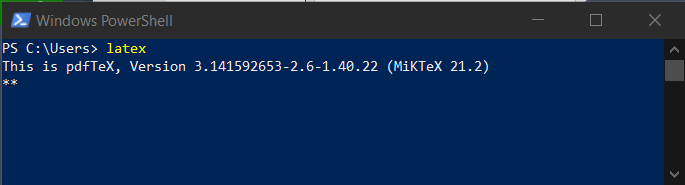
\includegraphics[width=0.75\textwidth]{Imagenes/guia01_1.png}
    \caption{Captura de una PowerShell ejecutando \LaTeX{} en Windows.}
\end{figure}


Al igual que cualquier lenguaje de programación, nuestro primer paso lo daremos con el clásico \textit{Hello Word} o \textit{Hola Mundo}, para ello seguiremos el siguiente ejemplo:

\vspace{6pt}

\begin{lstlisting}[frame=single]
\documentclass[10pt]{article}

\begin{document}
Hola Mundo
\end{document}
\end{lstlisting}

\begin{advertencia}
Para compilar un documento exitosamente se requiere que siempre exista contenido en el ambiente \verb@document@. Si intentamos compilar un documento vacío este proceso se detendrá sin resultado alguno.
\end{advertencia}

El archivo que contiene el código fuente posee la extensión \texttt{.tex} mientras que el archivo que contiene los registros del proceso de compilación poseen la extensión  \texttt{.log}. Una tabla completa con los archivos más usuales en la compilación de un documento se encuentran a continuación:

\begin{table}[H]
    \centering
    \begin{tabular}{ll}
        \hline
        \textbf{Tipo de archivo} & \textbf{Extensiones más comunes}  \\
        Código base &  \texttt{.tex} \\
        Base de datos para bibliografía & \texttt{.bib}\\
        Índice & \texttt{.ind}\\
        Imágenes & \texttt{.ps},\texttt{.eps},\texttt{.tif},\texttt{.png},\texttt{.jpg},\texttt{.gif},\texttt{.pdf}\\
        Clases  & \texttt{.cls}\\
        Paquetes & \texttt{.sty}\\
        Auxiliar & \texttt{.aux}\\
        Tabla de contenidos & \texttt{.toc}\\
        Lista de figuras\fs/\fs Tablas & \texttt{.lof},\texttt{.lot}\\
        Medidas del tipo & \texttt{.tfm}\\
        Transcripción & \texttt{.log}\\
        Índice alfabético & \texttt{idx},\texttt{.ind}\\
        TrueType & \texttt{.ttf}\\
        OpenType & \texttt{.otf}\\
        \hline
    \end{tabular}
    \caption{Tipos de archivos usados en \TeX{} y \LaTeX{}}
    \label{tab:2.1}
\end{table}


Regresando a la estructura del archivo fuente tenemos lo siguiente: 
El primer comando especifica la \textit{clase} de documento que vamos a generar y tiene la siguiente estructura:

\begin{lstlisting}[frame=single]
\documentclass[Opciones del documento]{Tipo de documento}
\end{lstlisting}

\noindent
Para el desarrollo de los ejemplos usaremos:

\begin{lstlisting}[frame=single]
\documentclass[10pt]{article}
\end{lstlisting}

Un documento básico en \LaTeX{} se compone de dos partes: el \textit{preámbulo} y el \textit{cuerpo}. El preámbulo, incluye la \emph{clase}\footnote{Una clase es un archivo de extensión \texttt{.cls} que define el formato del documento.} del documento, paquetes a usar y configuraciones adicionales, mientras que el cuerpo contiene el texto y fórmulas matemática que van a ser mostradas.


\begin{lstlisting}[frame=single]
% Preambulo
\documentclass[10pt]{article}

\usepackage[utf8]{inputenc}
\usepackage[T1]{fontenc}
\usepackage[spanish]{babel}
\usepackage{geometry}

\begin{document}
% Cuerpo
Hola Mundo
\end{document}
\end{lstlisting}

A continuación se encuentra una lista de las clases más usuales para crear documentos en \LaTeX{}

\begin{multicols}{3}
\begin{itemize}
    \item \verb@article@;
    \item \verb@report@;
    \item \verb@book@;
    \item \verb@slides@;
    \item \verb@beamer@;
    \item \verb@letter@;
    \item \verb@standalone@;
    \item \verb@minimal@.
\end{itemize}
\end{multicols}

Por otra parte, existen varias opciones a seleccionar dentro de una clase, la más común es el tamaño de la fuente. Los tamaños más usuales son:

\begin{multicols}{3}
\begin{itemize}
    \item \verb@10pt@;
    \item \verb@11pt@;
    \item \verb@12pt@.
\end{itemize}
\end{multicols}

\subsection{Paquetes básicos}

Un paquete \LaTeX{} es un archivo que incluye código \TeX{} con la intención de agregar nuevas funciones o facilitar otras ya existentes, los paquetes disponibles y su documentación se pueden encontrar en: \href{https://ctan.org/}{https://ctan.org/}. Para incluir un paquete, se usa la siguiente sintaxis:

\begin{lstlisting}[frame=single]
\usepackage[Opciones del paquete]{Nombre del paquete}
\end{lstlisting}

\noindent
Los paquetes básicos para comenzar a escribir en \LaTeX\hspace{1.5pt} son:

\begin{itemize}
    \item 
        \verb"inputenc": La opción \verb"utf8" nos permite agregar los acentos y símbolos codificados en formato \verb"utf-8" directamente desde nuestro teclado.
    \item
        \verb"fontenc": Permite la selección de una codificación de fuentes apropiada para el documento.
    \item
        \verb"babel": Indica el idioma del documento.
    \item
        \verb"geometry": Ajusta la geometría de la hoja.
\end{itemize}

\noindent
Con los paquetes mencionados es posible comenzar la composición de un documento, conforme avancemos en los contenidos introduciremos nuevos paquetes que ampliarán las herramientas con las que disponemos. No obstante, para el desarrollo de un documento se recomienda trabajar únicamente con los paquetes requeridos para evitar conflictos en la compilación del documento.

\subsection{Paquete \emph{babel}}

El paquete babel es una de las herramientas básicas para la composición de textos pues permite modificar el idioma del documento; En algunos casos este paquete puede ser reemplazado por el siguiente código que modifica «manualmente» los parámetros que normalmente serían modificados por \texttt{babel}

\begin{lstlisting}[frame=single]
\renewcommand{\contentsname}{Contenido}
\renewcommand{\partname}{Parte}
\renewcommand{\appendixname}{Ap\'endice}
\renewcommand{\figurename}{Figura}
\renewcommand{\tablename}{Tabla}
\AtBeginDocument{\renewcommand\tablename{Tabla}}
\renewcommand{\abstractname}{Resumen}
\renewcommand{\refname}{Bibliograf\'{\i}a}
\end{lstlisting}

\begin{advertencia}
En general, se recomienda usar los acentos con la forma \verb@\'@ en lugar del acento directo desde el teclado.
\end{advertencia}

\subsection{Paquete \emph{geometry}}

Una de las primeras tareas a realizar en la preparación de un documento es definir su tamaño, márgenes y otras medidas. Para la realización de esta tarea vamos a recurrir al paquete \texttt{geometry}, este nos permite modificar de manera sencilla todas las medidas del documento.


Por ejemplo, si deseamos cambiar el tamaño del papel a un tamaño A5, basta colocar el tamaño deseado como parte de las opciones del paquete:

\begin{lstlisting}[frame=single]
\usepackage[a5paper]{geometry}
\end{lstlisting}

Los tamaños disponibles son los siguientes:

\begin{table}[h]
  \begin{center}
  \begin{tabular}{ccccccc}
    a0paper & a1paper & a2paper & a3paper & a4paper & a5paper & a6paper \\ b0paper & b1paper & b2paper & b3paper & b4paper & b5paper &  b6paper \\ c0paper & c1paper & c2paper & c3paper & c4paper & c5paper & c6paper \\ 
    b0j & b1j & b2j & b3j& b4j& b5j& b6j \\
    ansiapape & ansibpaper & ansicpaper & ansidpaper & ansiepaper & letterpaper & executivepaper \\  legalpaper 
  \end{tabular}
 \end{center}
\end{table}

Por otra parte, los parámetros de medidas disponibles y más comunes son:

\begin{itemize}
    \item Ancho de texto (\texttt{textwidth})
    \item Altura de texto (\texttt{textheight})
    \item Margen superior (\texttt{top, tmargin})
    \item Margen inferior (\texttt{bottom, bmargin})
    \item Margen izquierdo (\texttt{left, lmargin, inner})
    \item Margen derecho (\texttt{right, rmargin, outer})
\end{itemize}

Existen opciones adicionales e información que puede ser consultada en la documentación del paquete, aunque un breve resumen se encuentra en la siguiente imagen:

\begin{figure}[H]
    \centering
    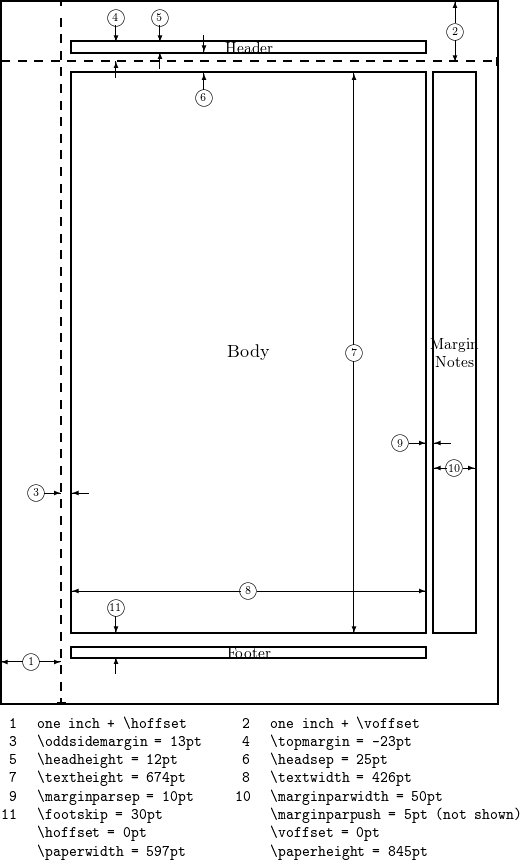
\includegraphics[width=0.75\textwidth]{Imagenes/Layout-dimensions.png}
\end{figure}

\section{Escritura de texto}

\subsection{Espacios}

\LaTeX \hspace{3pt} trata todos los caracteres en blanco, tales como el espacio en blanco o el tabulador, como un solo espacio. El espacio en blanco al principio de una linea se ignora, y un salto de linea aislado se trata como espacio en blanco. Una linea vacía entre dos lineas de texto define el fin de un párrafo. Varias lineas vacías se tratan igual que una sola linea vacía.


\subsubsection{Espacios Horizontal}

\LaTeX\hspace{1.5pt} determina los espacios entre palabras y oraciones automáticamente.  Para añadir espacio horizontal, se usa \verb|\hspace{|\emph{longitud}\verb|}|. Si el espacio debiera mantenerse incluso si cae al final o al principio de renglón, use \verb|\hspace*| en  lugar de \verb|\hspace|.
\noindent
La \emph{longitud} en el caso más simple es sólo un número más una unidad.  Las unidades más importantes se listan en el cuadro~\ref{units}.

\begin{table}[h]
 \caption{\TeX \hspace{1.5pt} Unidades.} \label{units}
  \begin{center}
  \begin{tabular}{@{}rl@{}}
    \texttt{mm}          & milímetro $\approx 1/25$~pulgada \\
    \texttt{cm}          & centímetro = 10~mm  \\
    \texttt{in}          & pulgada $=$ 25,4~mm \\
    \texttt{pt}          & punto $\approx 1/72$~pulgada $\approx \frac{1}{3}$~mm  \\
    \texttt{em}          & $\approx$ anchura de una `M' en la fundición actual \\
    \texttt{ex}          & $\approx$ altura de una `x' en la fundición actual \\
    \verb"\baselineskip" & altura de un salto de linea
  \end{tabular}
 \end{center}
\end{table}

\noindent
La orden \verb"\hfill" genera un espacio que se expande hasta llenar todo el espacio sobrante en un renglón o página.

\subsubsection{Espaciado Vertical}

El espacio entre párrafos, secciones, subsecciones,\ldots{}  lo determina automáticamente \LaTeX.  Si es necesario, un espacio vertical adicional \emph{entre dos párrafos} puede añadirse con la orden \verb|\vspace{|\emph{longitud}\verb|}|. Si el espacio debe preservarse en lo alto o en lo bajo de la página, use la versión  de la orden con asterisco, \verb|\vspace*|, en lugar de \verb|\vspace|. Espacio adicional entre dos lineas del \emph{mismo} párrafo o dentro de una tabla se indica con el comando \verb|\\[|\emph{longitud}\verb|]|

\subsubsection{Espacio duro}

En algunos casos se requiere colocar espacios pero estos no deben separarse en un salto de linea, estos se conocen como espacios duros o irrompibles pues de coincidir al final de una linea mueven todo el bloque de texto y no permiten que se separen. Para introducir este tipo de espacios usamos una virgulilla (\verb@~@).

\subsection{Caracteres especiales}

Los siguientes símbolos son caracteres reservados que tienen un significado especial en \LaTeX. Si los escribimos directamente, no se imprimirán, sino que obligarán a \LaTeX a hacer cosas que no se pretendía hacer.
 \begin{center}
  \verb.#  $  %  ^  &  _  {  }  ~  \ ". %$
 \end{center}

Se pueden usar algunos de estos caracteres añadiendo una barra invertida como prefijo:
 \begin{center}
  \verb.\# \$ \% \^{} \& \_ \{ \} \~{}.
 \end{center}
obteniendo así los símbolos: \# \$ \% \^{} \& \_ \{ \} \~{}.

Para la barra invertida se deberá escribir \verb@\backslash@. y la forma correcta de poner comillas es usar dos~\textasciigrave~(acentos graves) para abrirlas y dos~\textquotesingle~(apóstrofos) para cerraras.


\subsection{Alineación (\emph{flushleft}, \emph{flushright} y \emph{center})}

Los entornos \texttt{flushleft} y \texttt{flushright} generan párrafos alineados a la izquierda o a la derecha respectivamente. El entorno \texttt{center} genera texto centrado.

\subsection{Fundiciones y tamaños}

\LaTeX\hspace{1.5pt} escoge la fundición y el tamaño de fundición apropiados basándose en la estructura lógica del documento (secciones, notas al pie, \ldots).   Para cambiar fundiciones y tamaños se puede usar las órdenes listadas en los cuadros~\ref{fonts} y~\ref{sizes}. El cuadro~\ref{tab:pointsizes}
muestra los tamaños absolutos en puntos para estas órdenes según se implementan en las clases de documentos normales.

\begin{table}[H]                                                           
\caption{Fundiciones.} \label{fonts}
 \begin{center}
  \begin{tabular}{@{}rl@{\qquad}rl@{}}
    \hline
    \verb|\textrm{...}|        &      \textrm{{rematada}}&
    \verb|\textsf{...}|        &      \textsf{{palo seco}}\\
    \verb|\textmd{...}|        &      \textmd{peso medio}&
    \verb|\textbf{...}|        &      \textbf{{negrita}}\\
    \verb|\textup{...}|        &       \textup{{recta}}&
    \verb|\textit{...}|        &       \textit{{cursiva}}\\
    \verb|\textsl{...}|        &       \textsl{{oblicua}}&
    \verb|\textsc{...}|        &       \textsc{{Versalitas}}\\
    \verb|\emph{...}|          &            \emph{destacada} &
    \verb|\texttt{...}|        &      \texttt{de máquina}\\\hline
  \end{tabular}
 \end{center}
\end{table}

\begin{table}[H]
\index{font size}
\caption{Tamaños de fundición.} \label{sizes}
\begin{center}
\begin{tabular}{@{}ll}
\hline
\verb"\tiny"      & \tiny        tiny\\
\verb"\scriptsize"   & \scriptsize  scriptsize\\
\verb"\footnotesize" & \footnotesize  footnotesize\\
\verb"\small"        &  \small          small\\
\verb"\normalsize"   &  \normalsize  normalsize \\
\verb"\large"        &  \large       large\\
\verb"\Large"        &  \Large       Large \\[5pt]
\verb"\LARGE"        &  \LARGE       LARGE \\[5pt]
\verb"\huge"         &  \huge        huge \\[5pt]
\verb"\Huge"         &  \Huge        Huge\\[5pt]\hline
\end{tabular}
\end{center}
\end{table}

\begin{table}[H]
\caption{Tamaños absolutos en puntos para las clases normales.}\label{tab:pointsizes}
\label{tab:sizes}
\begin{center}
\begin{tabular}{lrrr}
\hline
\multicolumn{1}{c}{\textbf{tamaños}} &
\multicolumn{1}{c}{\textbf{10pt (por omisión) }} &
           \multicolumn{1}{c}{\textbf{opción 11pt}}  &
           \multicolumn{1}{c}{\textbf{opción 12pt}}\\
\verb|\tiny|       & 5pt  & 6pt & 6pt\\
\verb|\scriptsize| & 7pt  & 8pt & 8pt\\
\verb|\footnotesize| & 8pt & 9pt & 10pt \\
\verb|\small|        & 9pt & 10pt & 11pt \\
\verb|\normalsize| & 10pt & 11pt & 12pt \\
\verb|\large|      & 12pt & 12pt & 14pt \\
\verb|\Large|      & 14pt & 14pt & 17pt \\
\verb|\LARGE|      & 17pt & 17pt & 20pt\\
\verb|\huge|       & 20pt & 20pt & 25pt\\
\verb|\Huge|       & 25pt & 25pt & 25pt\\\hline
\end{tabular}
\end{center}
\end{table}



\section{Otros comandos}

A continuación se encuentra una pequeña lista de otros comandos útiles en el desarrollo de documentos:

\begin{itemize}
    \item \verb@\renewcommand{\baselinestretch}{1.5}@ Modificación del interlineado
    \item \verb@\pagestyle{empty}@ Eliminar numeración de página
    \item \verb@\parindent=0mm@ Eliminar las sangría
    \item \verb@\newpage@ Agrega una nueva página
    \item \verb@\pagebreak@ Inserta un salto de página
    \item \verb@\today@ Imprime la fecha actual
\end{itemize}


\subsection{Separación de palabras}

En general,con el paquete babel aseguramos que la mayoría de las palabras se separen correctamente. Sin embargo, es posible que algunas palabras no se separen correctamente, para subsanar este error podemos especificar la forma para separar las palabras de la siguiente manera:

\begin{lstlisting}[frame=single]
Electroence\-falografista
\end{lstlisting}

Así, esto produce el siguiente resultado:

\begin{center}
{ \fboxsep 12pt
\fcolorbox {black}{white}{
\begin{minipage}[t]{2cm}
Electroence\-falografista
\end{minipage}
} }
\end{center}

\end{document} 